\chapter[Lezione X]{Lezione X\newline\small{\emph{26/05/2011}}}
	\section{Breve storia dell'informatica}
L'\emph{informatica} è una disciplina che si fonda su due pilastri fondamentali:
\begin{description}
	\item[Teoria della computazione] (Turing, Church, Post nel 1936) che si occupa di studiare il concetto di \emph{algoritmo} e tutto ciò che ne consegue;
	\item[Teoria dell'informazione] (Shannon nel 1949) che nasce essenzialmente dal problema di trasportare messaggi da un luogo ad un altro nel modo più sicuro ed efficiente possibile.
\end{description}

		\subsection{Teoria della computazione}
La \emph{teoria della computazione} nasce dalla domanda: cosa è possibile calcolare meccanicamente?

Parte della teoria si spende nello specificare innanzitutto il significato della parola <<meccanicamente>>.
Data la generalità di questa trattazione, si può assumere che significhi <<seguendo delle istruzioni fisse>>.

		\subsection{La macchina di Turing}
		\label{subsec:mturing}
Già negli anni '30 esistevano le calcolatrici ma la tecnologia non aveva ancora prodotto niente di più avanzato.
C'erano,\marginpar{Computer} tuttavia i \emph{computer}\index{computer} che, in lingua inglese, erano i \emph{contabili}.

Alan Mathison Turing (vedi il paragrafo~\ref{subsec:turing} a pagina~\pageref{subsec:turing}) s'ispirò proprio al modo di lavorare del contabile per mettere a punto la sua idea si calcolatore.
Questi esegue dei calcoli applicando formule date a priori, una matita ed un foglio a quadretti.
Non gli sono richieste creatività o inventiva; svolge solo dei calcoli e, di tanto in tanto, si serve del foglio e della matita per appuntare dei risultati intermedi.
Il contabile ha a disposizione una quantità finita di segni differenti da poter usare: riesce a riconoscere ed interpretare un numero finito di simboli.
Anche il foglio di cui dispone ha una dimensione limitata e in ogni quadretto c'è spazio per un solo simbolo.
Inoltre il numero delle \emph{condizioni interne}, o come Turing stesso li definì <<stati mentali>>, che gli permettono di reagire in modo diverso agli stimoli esterni in cui può trovarsi è finito.

\begin{wrapfloat}{figure}{i}{0pt}
%	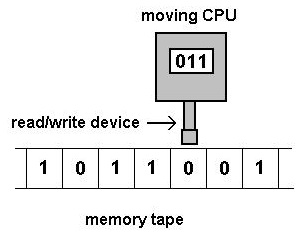
\includegraphics[width=0.5\columnwidth]{immagini/turing}
\begin{minipage}{.5\columnwidth}
	\centering
% Turing Machine
% Author: Sebastian Sardina

\usetikzlibrary{chains,fit,shapes}

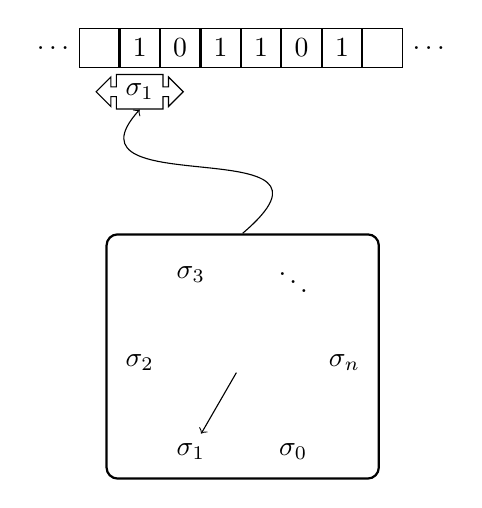
\begin{tikzpicture}
%\tikzstyle{every path}=[very thick]

\edef\sizetape{0.5cm}
\tikzstyle{tmtape}=[
	draw,
	minimum size=\sizetape,
%	fill pattern=dots
]
\tikzstyle{tmhead}=[
	arrow box,
	draw,
	minimum size=.4cm,
	arrow box
	arrows={east:.25cm, west:0.25cm}
]

%% Draw TM tape
\begin{scope}[
	start chain=1 going right,
	node distance=0mm
]
    \node [on chain=1,tmtape,draw=none] {$\dots$};
    \node [on chain=1,tmtape] {};
    \node [on chain=1,tmtape] (input) {\num{1}};
    \node [on chain=1,tmtape] {\num{0}};
    \node [on chain=1,tmtape] {\num{1}};
    \node [on chain=1,tmtape] {\num{1}};
    \node [on chain=1,tmtape] {\num{0}};
    \node [on chain=1,tmtape] {\num{1}};
    \node [on chain=1,tmtape] {};
    \node [on chain=1,tmtape,draw=none] {$\dots$};
%    \node [on chain=1,above,midway] {\textbf{Input/Output Tape}};
\end{scope}

%% Draw TM Finite Control
\begin{scope}[
	shift={(2.4cm,-4cm)},
	start chain=circle placed {at=(-\tikzchaincount*60:1.3)}
]
\foreach \i in {\sigma_0,\sigma_1,\sigma_2,\sigma_3,\ddots,\sigma_n}
	\node [on chain] {$\i$};

% Arrow to current state
\node (center) {};
\draw[->] (center) -- (circle-2);

\node[
	rounded corners,
	draw=black,
	thick,
	fit=(circle-1) (circle-2) (circle-3) (circle-4) (circle-5) (circle-6),
%	label=below:\textbf{Finite Control}
] (fsbox) {};
\end{scope}

%% Draw TM head below (input) tape cell
\node [tmhead,yshift=-.3cm] at (input.south) (head) {$\sigma_1$};

%% Link Finite Control with Head
\path[->,draw] (fsbox.north) .. controls (4.,-1) and (0,-2) .. node[right] 
			(headlinetext)
 			{} 
			(head.south);
%\node[xshift=3cm] at (headlinetext)  
%			{\begin{tabular}{c} 
%				\textbf{Reading and Writing Head} \\  
%				\textbf{(moves in both directions)} 
%			 \end{tabular}};

\end{tikzpicture}

	\caption{Macchina di Turing.}
	\label{fig:tm}
\end{minipage}
\end{wrapfloat}
Prendendo \marginpar{Macchina di Turing} le mosse da questi presupposti, Turing immaginò la cosiddetta \emph{Macchina di Turing} stilizzata in figura~\ref{fig:tm}.
Molto schematicamente, si tratta di una scatola che può trovarsi in un numero finito di stati interni differenti.
Dalla scatola si protende un braccio che dà su un nastro scorrevole il quale può contenere numeri, caratteri alfanumerici o caselle vuote.
Il nastro può essere allungato indefinitamente, pur restando di lunghezza finita.
Il braccio è in grado sia di leggere dal nastro che di scrivervi sopra.
Il cuore dell'apparecchio è la \emph{tabella delle istruzioni}.

Sia\marginpar{Alfabeto e istruzioni} $S\coloneqq \Set{\sigma_1,\sigma_2,\dots,\sigma_n}$ l'insieme degli stati interni assumibili dalla macchina e $A\coloneqq\Set{\alpha_1,\alpha_2,\dots,\alpha_m}$, con $n,m\in\N$ l'insieme dei simboli che essa riesce a riconoscere.
%\[
%\left[
%	\begin{aligned}
%S &= \{ \sigma_1, \dots, \sigma_n \}; \\
%A &= \{ \alpha_1, \dots, \alpha_m \};
%	\end{aligned}
%\right.
%\text{ con } m,n \in \mathbb{N}.
%\]
Le istruzioni della macchina, allora, hanno la forma:
\begin{quote}
<<Se \MyComment{il tuo stato è $\sigma_i$} e se \MyComment{leggi $\alpha_e$ nella casella}; allora \MyComment{cambia stato $\sigma_i\mapsto\sigma_r$} e \MyComment{sposta la testina a destra} e \MyComment{scrivi $\alpha_k$}\dots>>
\end{quote}
Ad un certo punto, la macchina troverà un'istruzione di \MyComment{stop} e si fermerà.
Allora si possono fissare gli insiemi dell'alfabeto $A$ e degli stati interni $S$ (ossia delle istruzioni):
\begin{description}
	\item[Alfabeto] codice binario;
	\item[Istruzioni] Immaginando che il nastro scorra verso sinistra, si possono definire i seguenti stati interni:
		\begin{enumerate}
			\item
Se \MyComment{la testina legge una cifra}, allora \MyComment{va a destra};
			\item
Se \MyComment{la testina legge una casella vuota} allora \MyComment{scrive la cifra \num[detect-all]{0} nella casella}.
		\end{enumerate}
\end{description}
In pratica, tale funzione aggiunge uno zero in coda ad un numero binario, che corrisponde a raddoppiarlo.

		\subsection{Problemi insolubili}
		\label{subsec:ins}

Con questo tipo di macchine è possibile calcolare funzioni $f\colon\N\to\N$ come, ad esempio, $f(n)\coloneqq2n$, $f(n)\coloneqq\sqrt{n}$ (purché ci si accontenti della sola parte intera), $f(n)\coloneqq n^2+n+1$, etc\dots{}
Esistono, tuttavia, delle funzioni che non possono essere calcolate con una macchina di Turing dal momento che non esiste un processo meccanico (algoritmo) che porti alla loro soluzione.\footnote{Questo si può dimostrare provando che l'insieme funzioni aritmetiche calcolabili è un sottoinsieme di quello delle funzioni aritmetiche.
Dal momento che una funzione aritmetica è calcolabile se e solo se esiste un algoritmo che la calcola \cite{fp:comp}, segue la tesi.}

Non \marginpar{Polinomio di grado qualsiasi} esiste un algoritmo che, dato un polinomio a coefficienti interi di grado non fissato a priori, sia in grado di stabilire se esistano o meno delle radici intere.
Tale risultato è ottenibile solo conoscendo in anticipo il grado del polinomio.


Un'altra \marginpar{Problema dell'arresto} questione non risolubile è il cosiddetto \emph{problema dell'arresto}.
Si consideri un codice del tipo:
\begin{lstlisting}
i = 1;
while( i > 0 )
	i ++;
\end{lstlisting}
Esso genera un ciclo teoricamente infinito che, una volta avviato, non può arrestarsi se non interrotto dall'esterno.
%\footnote{Vedi: ``black out'', oppure ``utente incavolato che sfascia il computer perché il suo programmino non funziona''\dots}
Dopo aver compilato il programma, non c'è alcuna possibilità d'individuare un errore di questo tipo durante l'esecuzione: non si può dimostrare di aver scritto un ciclo infinito. %(anche se ad un certo punto, cominciano a sorgere forti sospetti\dots).
Si potrebbe pensare, allora, di scrivere un programma che verifichi il codice di un altro dal punto di vista logico.
Lo stesso Turing dimostrò che un siffatto programma non può essere steso.

		\subsection{La macchina universale}
Presa una macchina di Turing tale con stati interni $S=\Set{\sigma_1, \sigma_2, \sigma_3}$ e alfabeto $A=\Set{1, 0}$ tale che siano assegnate istruzioni della forma
\begin{equation}\label{eq:istruzione}
%	\begin{aligned}	
%	&\left[
%		\begin{aligned}
%&S=\{\sigma_1, \sigma_2, \sigma_3\}; \\
%&A=\{1, 0\};	\\
%		\end{aligned}
%	\right .	\\
%&
(\sigma_1, 0) \mapsto (1, \sigma_2, \text{ destra}),	%\\
%&\vdots
%	\end{aligned}
\end{equation}
si possono ricavare i corrispondenti stati interni del computer usando il suo alfabeto (il codice binario).
Nello specifico, ci sono tre stati  (che sono \num[parse-numbers=false]{11_2} in binario) e due (ossia \num[parse-numbers=false]{10_2}) simboli.
\begin{table}
	\centering
\subfloat[][{Istruzioni.}\label{tab:istr}]{
	\begin{tabular}{l S}
		\toprule
\emph{Istruzione}			&{\emph{Numero}}	\\
		\midrule
Sposta la testina a destra		&0	\\
Sposta la testina a sinistra		&1	\\
		\bottomrule
	\end{tabular}
}\qquad
\subfloat[][{Stati interni.}\label{tab:stat}]{%}
	\begin{tabular}{l S[parse-numbers=false]}
		\toprule
\emph{Stato}			&{\emph{Numero}}	\\
		\midrule
$\sigma_1$				&01	\\
$\sigma_2$				&10	\\
$\sigma_3$				&11	\\
		\bottomrule
	\end{tabular}
}
	\caption[Macchina di Turing]{Convenzioni binarie per la macchina di Turing.}
\end{table}
Adottando le convenzioni delle tabelle~\ref{tab:istr} e~\ref{tab:stat} è possibile tradurre le istruzioni in linguaggio binario.
Gli stati vengono mappati nell'insieme $\Set{01,10,11}$ e l'alfabeto diventa $\Set{1,0}$, pertanto l'istruzione~\eqref{eq:istruzione} si traduce in
\begin{equation}\label{eq:istruzione-bin}\tag{\ref*{eq:istruzione}/bin.}
%	\begin{aligned}	
%	&\left[
%		\begin{aligned}
%&\mathtt{01\ 10\ 11} 		\\
%&\mathtt{1\ 0} 			\\
%		\end{aligned}
%	\right .	\\
\mathtt{1\_0\_1\_10\_0}%	\\
%&\vdots
%	\end{aligned}
\end{equation}
Il problema di distinguere i numeri da elaborare dalle istruzioni è facilmente risolvibile.

Ora, una macchina di Turing può essere descritta con un numero.
Si consideri, allora, una macchina $U$ che riesca a riconoscere parti di codice di altre due macchine $E\colon f(x)\coloneqq2x$ e $D\colon f(x)\coloneqq x^2-1$.
Se alla macchina $E$ corrisponde il codice~\eqref{eq:istruzione-bin} della moltiplicazione per due, la macchina $U$ riesce ad interpretarlo come istruzione ed applicarlo ad un numero $x$ (\num[parse-numbers=false]{101}, ad esempio).
La macchina $U$ è una cosiddetta \emph{macchina universale}\index{macchina universale}.
In questo modo non c'è bisogno di progettare un apparecchio specifico per ogni algoritmo da eseguire ma ne basta uno solo.


Da \marginpar{La tesi di Church-Turing} quanto detto finora, discende la
\begin{thesis*}[di Church-Turing]
Le funzioni calcolabili dalla macchina di Turing sono \emph{tutte e sole} quelle calcolabili meccanicamente.
\end{thesis*}
Si noti che questo \emph{non} è un teorema perché discende direttamente da tutta la teoria ``costruita'' da Turing.


Gli studi di John von Neumann negli anni '40 (vedi il paragrafo~\ref{sec:neu} a pagina~\ref{sec:neu}) si basavano proprio sulle osservazioni di Turing.


	\section{Algoritmo di Dijkstra per i cammini minimi}

Un \emph{grafo}\index{grafo} (vedi il paragrafo~\ref{subsec:grafo} a pagina~\pageref{subsec:grafo}) è un oggetto composto di vertici\index{vertice}, o \emph{nodi}\index{nodo}, e lati\index{lato}, o \emph{archi}\index{arco}, che uniscono due nodi.


Siano $V=\Set{(x_1,y_1),\dots,(x_n,y_n)}$ ed $E\subseteq V\times V$ rispettivamente gli insiemi dei vertici e lati. 
Se si associa ad $e_{i}\in E$ un numero $z_i\in\R^+$, è naturale interpretare $z_i$ come la distanza che intercorre tra i due nodi collegati dall'arco $e_i$.
Dato un grafo, è dunque lecito chiedersi quale sia il cammino \emph{minimo}, o di \emph{minimo costo}, tra due suoi vertici qualsiasi.
L'\algo{algoritmo di Dijkstra} risponde a tale domanda.

\begin{figure}
	\centering
%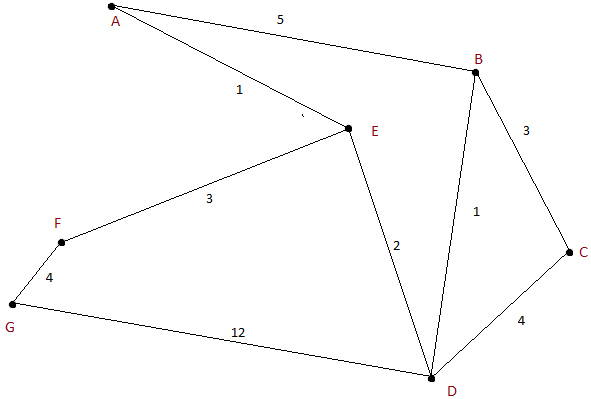
\includegraphics[width=\columnwidth]{immagini/dijkstra}
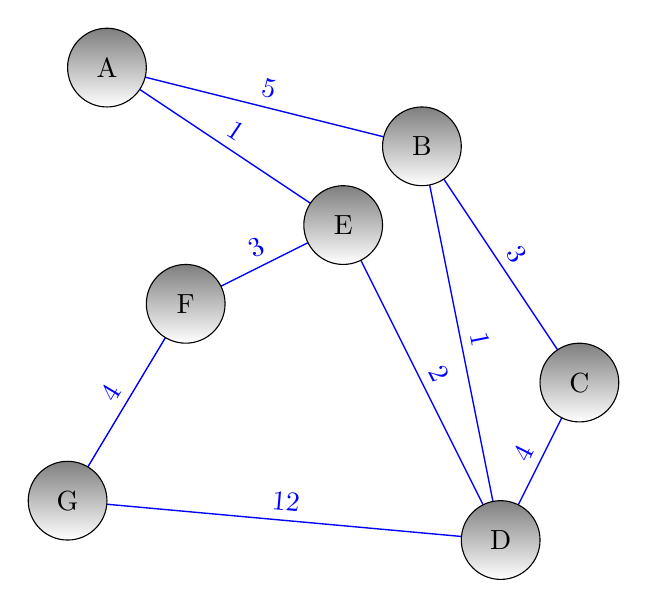
\begin{tikzpicture}
	\coordinate (A) at (-2,6);
	\coordinate (B) at (2,5);
	\coordinate (C) at (4,2);
	\coordinate (D) at (3,0);
	\coordinate (E) at (1,4);
	\coordinate (F) at (-1,3);
	\coordinate (G) at (-2.5,0.5);

	\foreach \a/\b/\d in {A/B/5, B/C/3, C/D/4, D/G/12, G/F/4, F/E/3, A/E/1, D/E/2, D/B/1}
		\draw [line width=0.5pt, color=blue] (\a) -- (\b) node [blue, sloped,midway,above] {$\d$};

	\foreach \n in {A,B,C,D,E,F,G} 
		\draw [] node [circle,draw,minimum size=1cm,top color=gray] at (\n) {\color{black}{\n}};

\end{tikzpicture}
	\caption{Rappresentazione grafica di un grafo.}
	\label{fig:dij}
\end{figure}
Si vuole calcolare il cammino più breve che collega il vertice~$A$ %\hyperlink{coordinate:A}{A}
della figura~\ref{fig:dij} con tutti gli altri.
\begin{table}
	\centering
\caption{La tabella contiene alcune distanze partendo dal vertice $A$. Il cammino minimo è evidenziato.}
\label{tab:dij}
\begin{tabular}{l l l}
	\toprule
\emph{Vertice}	&\emph{Distanza}		&\emph{Percorso}		\\
	\midrule
$A$ 			&0			& /					\\
$B$ 			&\textbf{5}		&$\mathbf{AB}$			\\
$C$ 			&8; \textbf{7}	&$ABC; \mathbf{AEDC}$		\\
%$D$ 		&12; 6; \textbf{3}	&$ABCD; ABD;\mathbf{AED}$	\\
%$E$ 		&\textbf{1}		&$\mathbf{AE}$			\\
\vdots 		&\vdots 		& \vdots 				\\
	\bottomrule
\end{tabular}
\end{table}
Per fare ciò è conveniente registrare tutti i possibili percorsi (con le rispettive distanze) in una tabella come la~\ref{tab:dij}.
Si trovano i nodi immediatamente vicini ad~$A$. %\hyperlink{coordinate:A}{$A$}.
Si ha che $\overline{AB}=5$ e $\overline{AE}=1$.
Per ora, queste sono le distanze minime.
Partendo ora da~$B$%\hyperlink{coordinate:B}{$B$}
, si ha che $\overline{AC}=\overline{AB}+\overline{BC}=8$ e $\overline{AD}=\overline{AB}+\overline{BC}=6$.
Entrambi questi percorsi individuano, al momento, dei cammini minimi.
Ripetendo l'operazione per tutti i vertici del grafo, si ottiene tabulata la distanza minima tra~$A$%\hyperlink{coordinate:A}{$A$}
 e qualsiasi altro nodo (ma anche tra due vertici qualsiasi $v_1,v_2\in\Set{A, B, C, D, E, F, G}$).


Per \marginpar{Rappresentazioni in \lang{C}} tradurre tale algoritmo in linguaggio \lang{C}, c'è innanzitutto bisogno di trovare una rappresentazione per il grafo.
Vi sono diverse soluzioni:
\begin{itemize}
	\item
Si rappresentano i vertici con degli interi e il lati con un record che contenga informazioni sui nodi che collega e la loro distanza;
	\item
Si usa una matrice.

\begin{table}
	\centering
\caption[Rappresentazione matriciale di un grafo.]{Rappresentazione di un grafo con una matrice quadrata $n$-dimensionale. I valori nulli sulla diagonale indicano che nessun arco collega un vertice con se stesso.}
\label{tab:mat}

\begin{tabular}{>$c<$ | S S S S}
		&{$v_1$}		&{$v_2$}		&{$\dots$} 	&{$v_N$} 		\\
		\midrule
v_1		&0		&4.5		&{$\dots$} 	&0		\\
v_2		&3		&0		&{} 	&5.7		\\
\vdots 	&{\vdots} 	&{} 	&{$\ddots$} 	&{$\vdots$} 	\\
v_ N		&8.9		&0		&{$\dots$} 	&0		\\
	\end{tabular}
\end{table}
Avendo dei vertici $v_{i\in\{1,\dots,N\}}\in V$, si dichiara una matrice $N\times N$ come la tabella~\ref{tab:mat} e si stabilisce che:
	\begin{itemize}
		\item
Se tra due vertici c'è un lato, si scrive nella casella corrispondente il valore $1$ (o la distanza $z\in\mathbb{R^{+}}$);
		\item
Se tra due vertici non c'è un lato, si scrive nella casella corrispondente il valore $0$.
	\end{itemize}
Si noti che, avendo dichiarato una matrice $\Set{m_{ij}}$ (di tipo \lstinline!float!), gli elementi diagonali $m_{jj}$ sono nulli se non esistono archi che collegano un punto con se stesso, come in figura~\ref{fig:dij}.
Con questa rappresentazione, il costo computazionale dell'algoritmo di Dijkstra (siccome sulla diagonale ci sono solo valori nulli) è
\begin{equation}
c_\textup{D}(N) = N(N-1)\underset{N\to\infty}{\thicksim} N^2.
\end{equation}
Pertanto, la rappresentazione matriciale risulta piuttosto scomoda se il grafo è sparso, cioè se ci sono pochi archi.
	\item
Ci si serve di una \emph{lista adiacenze}.


\begin{figure}
	\centering
\subfloat[][Gli archi del grafo non sono orientati pertanto la matrice è simmetrica e tutte le informazioni sono contenute nella parte sopra, o sotto, la diagonale (compresa).]{
	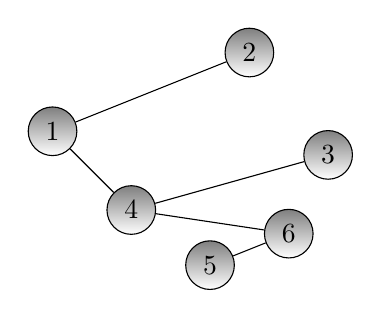
\begin{tikzpicture}
\begin{scope}[
	every node/.append style = {
		circle,
		draw,
%		minimum size=1cm,
		top color=gray
	}
]
\node (1) at (0,0) {$1$};
\node (2) at (2.5,1) {$2$};
\node (4) at (1,-1) {$4$};
\node (5) at (2,-1.7) {$5$};
\node (3) at (3.5,-.3) {$3$};
\node (6) at (3,-1.3) {$6$};
\end{scope}

\draw (1) -- (2);
\draw (1) -- (4);
\draw (4) -- (3);
\draw (4) -- (6);
\draw (6) -- (5);
\end{tikzpicture}\quad

\begin{comment}
\def\d{1} %horizontal displacement
\def\vd{1}
% vertices linked to 1
\node (1q1) at (5,0*\vd) {$1$};
\node (4q1) at ($(1q1) + (\d,0)$) {$4$};
\node (2q1) at ($(4q1) + (\d,0)$) {$2$};

% vertices linked to 2
\node (1q2) at (5,-1*\vd) {$2$};
\node (1q2) at ($(1q2) + (\d,0)$) {$1$};

% vertices linked to 3
\node (1q3) at (5,-2*\vd) {3};
\node (4q3) at ($(1q3) + (\d,0)$) {4};

% vertices linked to 4
\node (1q4) at (5,-3*\vd) {4};
\node (3q4) at ($(1q4) + (\d,0)$) {3};
\node (1q4) at ($(3q4) + (\d,0)$) {1};
\node (6q4) at ($(1q4) + (\d,0)$) {6};

% vertices linked to 5
\node (1q5) at (5,-4*\vd) {5};
\node (6q5) at ($(1q5) + (\d,0)$) {6};

% vertices linked to 1
\node (1q6) at (5,-5*\vd) {6};
\node (4q6) at ($(1q6) + (\d,0)$) {4};
\node (5q1) at ($(4q6) + (\d,0)$) {5};
\end{comment}

\begin{tikzpicture}
\matrix (B) [
	matrix of math nodes,
	%nodes = {node style ge},,
	column sep=.7cm,
	row sep = 1pt,
	nodes={
		fill=blue!15
	},
] at (0,0) {
\node[fill=none] {\phantom{0}};\\
1	&4	&2	\\
2 &1 \\
3	&4\\
4	&3	&1	&6\\
5	&6\\
6	&4	&5\\
};

\foreach \x in {2,3,...,7}
	\draw [->] (B-\x-1.east) -- (B-\x-2.west);

\foreach \x in {2,5,7}
	\draw [->] (B-\x-2.east) -- (B-\x-3.west);

\draw  [->] (B-5-3.east) -- (B-5-4.west);
\end{tikzpicture}\quad
\begin{tikzpicture}
\matrix (A) [
	matrix of math nodes,
	%nodes = {node style ge},,
	column sep=3pt,
	row sep = 1pt
] at (10,0) { &1	&2	&3	&4	&5	&6 \\
1 &0 &1 &0	&1 &0 &0  \\
2  & &0 &0	&0 &0 &0  \\
 3 & & &0	&1 &0 &0  \\
 4 & & &	&0 &0 &1 \\
 5 & & &	& &0 &1 \\
 6 &\phantom{0} & &	& & &0 \\
};

\draw [color=black!20] (A-1-2.south west) node [] {} to (A-1-7.south east) ;
\draw [color=black!20] (A-2-2.north west) node [] {} to (A-7-2.south west) ;

\end{tikzpicture}
}

\subfloat[][Gli archi del grafo sono orientati pertanto la matrice \emph{non} è più simmetrica.
Inoltre gli elementi della diagonale non sono tutti nulli perché il nodo~$3$ è collegato a se stesso.]{
	\begin{tikzpicture}
\begin{scope}[
	every node/.append style = {
		circle,
		draw,
%		minimum size=1cm,
		top color=gray
	}
]
\node (1) at (0,0) {$1$};
\node (2) at (2.5,1) {$2$};
\node (4) at (1,-1) {$4$};
\node (5) at (2,-1.7) {$5$};
\node (3) at (3.5,-.3) {$3$};
\node (6) at (3,-1.3) {$6$};
\end{scope}

%%%%%%%%%%%%%%%%%%%%%%%%%%%%%%%%
% Arc from 3 to itself
\coordinate (O) at ($(3) + (0,.4)$);
\coordinate (A) at ($(3.north east)$);
\coordinate (B) at ($(3.north west)$);

\tikzset{
	compass style/.append style={
		->,
		shorten >= 1pt,
		shorten <= 1pt,
		color=black
		}
	}
\tkzCalcLength(O,B)\tkzGetLength{radius}
\tkzDrawArc[black, ->, R with nodes](O,\radius pt)(A,B)
%%%%%%%%%%%%%%%%%%%%%%%%%%%%%%%%

\begin{scope}[shorten >= 1pt, shorten <= 1pt]
\begin{scope}[->]
\draw (1) -- (2);
\draw (1) -- (4);
\draw (4) -- (3);
\draw (4) -- (6);
\draw (5) -- (6);

%\tkzDefPoint($(3.north) + (0,.5)$) {center};
%\tkzDrawArc[color=blue]( center,3.north east ) (3.north west);
%\draw (3.north east) .. controls ($(3.north) + (0,1)$) .. (3.north west);
\end{scope}

\draw[<->] (5) -- (2);
\end{scope}
\end{tikzpicture}\quad

\begin{comment}
\def\d{1} %horizontal displacement
\def\vd{1}
% vertices linked to 1
\node (1q1) at (5,0*\vd) {$1$};
\node (4q1) at ($(1q1) + (\d,0)$) {$4$};
\node (2q1) at ($(4q1) + (\d,0)$) {$2$};

% vertices linked to 2
\node (1q2) at (5,-1*\vd) {$2$};
\node (1q2) at ($(1q2) + (\d,0)$) {$1$};

% vertices linked to 3
\node (1q3) at (5,-2*\vd) {3};
\node (4q3) at ($(1q3) + (\d,0)$) {4};

% vertices linked to 4
\node (1q4) at (5,-3*\vd) {4};
\node (3q4) at ($(1q4) + (\d,0)$) {3};
\node (1q4) at ($(3q4) + (\d,0)$) {1};
\node (6q4) at ($(1q4) + (\d,0)$) {6};

% vertices linked to 5
\node (1q5) at (5,-4*\vd) {5};
\node (6q5) at ($(1q5) + (\d,0)$) {6};

% vertices linked to 1
\node (1q6) at (5,-5*\vd) {6};
\node (4q6) at ($(1q6) + (\d,0)$) {4};
\node (5q1) at ($(4q6) + (\d,0)$) {5};
\end{comment}

\begin{tikzpicture}
\matrix (B) [
	matrix of math nodes,
	%nodes = {node style ge},,
	column sep=.7cm,
	row sep = 1pt,
	nodes={
		fill=blue!15
	},
] at (0,0) {
\node[fill=none] {\phantom{0}};\\
1	&4	&2	\\
2 &5 \\
3	&3\\
4	&6	&3	&\node[fill=none] {\phantom{6}};\\
5	&2	&6\\
6\\
};

\foreach \x in {2,3,...,6}
	\draw [->] (B-\x-1.east) -- (B-\x-2.west);

\foreach \x in {2,5,6}
	\draw [->] (B-\x-2.east) -- (B-\x-3.west);

%\draw  [->] (B-5-3.east) -- (B-5-4.west);
\end{tikzpicture}\quad
\begin{tikzpicture}
\matrix (A) [
	matrix of math nodes,
	%nodes = {node style ge},,
	column sep=3pt,
	row sep = 1pt
] at (10,0) {
&1	&2	&3	&4	&5	&6 \\
1 &0 &1 &0	&1 &0 &0  \\
2  &0 &0 &0	&0 &1&0  \\
 3 &0 &0 &1	&0 &0 &0  \\
 4 &0 &0 &1	&0 &0 &1 \\
 5 &0 &1 &0	&0 &0 &1 \\
 6 &0 &0 &0	&0 &0 &0 \\
};

\draw [color=black!20] (A-1-2.south west) node [] {} to (A-1-7.south east) ;
\draw [color=black!20] (A-2-2.north west) node [] {} to (A-7-2.south west) ;

\end{tikzpicture}
}
	\caption[Lista adiacenze]{Grafo con rappresentazione per lista adiacenze e matriciale.}
	\label{fig:adi}
\end{figure}
Essa, come mostra la figura~\ref{fig:adi}, consiste in più serie di record ognuna delle quali si riferisce ad un nodo di partenza differente.
Ogni struttura contiene un campo che tenga traccia del nome del nodo collegato e un campo puntatore alla struttura successiva.
Nel campo puntatore dell'ultimo record si pone il valore \lstinline!NULL!.

Tale rappresentazione risulta piuttosto ridondante per grafi non orientati perché si usano due record per ogni arco, ma diventa più efficiente nel caso di grafi orientati.
Si noti che, volendo aggiungere il peso di ogni lato, si dovrebbe aggiungere ad ogni record un campo dedicato.
\end{itemize}